\documentclass[table]{beamer}

\mode<presentation>
{
  \definecolor{kardinalblue}{RGB}{77,106,255}

  \useoutertheme[subsection=false]{miniframes}
  \usecolortheme[named=kardinalblue]{structure}
  \useinnertheme{circles}
  \setbeamerfont{block title}{size=\normalsize}
  \usecolortheme{orchid}
  \setbeamerfont{frametitle}{series=\bfseries}
  \setbeamerfont{title}{series=\bfseries}
  \setbeamercovered{transparent}

  %%% le foot pour avoir la numérotation des slides %%%
  \setbeamertemplate{footline}{%
    \leavevmode%
    \hbox{%
      \begin{beamercolorbox}[wd=.5\paperwidth,ht=2.5ex,dp=1.125ex,
        leftskip=.3cm plus1fill,rightskip=.3cm]{author in head/foot}%
        \usebeamerfont{title in head/foot}\insertshorttitle
      \end{beamercolorbox}%
      \begin{beamercolorbox}[wd=.5\paperwidth,ht=2.5ex,dp=1.125ex,
        leftskip=.3cm,rightskip=.3cm plus1fil]{title in head/foot}%
        \usebeamerfont{author in head/foot}\insertshortauthor\hfill
        \insertframenumber/\inserttotalframenumber
      \end{beamercolorbox}%
    }%
    \vskip0pt%
  }

  \setbeamercolor{palette primary}{fg=white,bg=black}
  \setbeamercolor{palette secondary}{fg=white,bg=kardinalblue}
  \setbeamercolor{palette tertiary}{fg=white,bg=black}
  \setbeamercolor{palette quaternary}{fg=white,bg=kardinalblue}
}

\usepackage[utf8]{inputenc}
\usepackage{DejaVuSans}
\usepackage[T1]{fontenc}
\usepackage[english,french]{babel}
\usepackage{tikz}

\setbeamercovered{invisible}
\newcommand{\nologo}{\setbeamertemplate{logo}{}}

\newenvironment{foreignpar}[1][english]{%
    \em\selectlanguage{#1}%
}{}
\newcommand*{\foreign}[2][english]{%
    \emph{\foreignlanguage{#1}{#2}}%
}

\title[Un vaste voisinage pour les tournées de véhicules]{Un vaste voisinage pour le problème de tournées de véhicules}

\author{Guillaume Pinot}

\institute% (optional, but mostly needed)
{ Kardinal, Paris, France }
%% - Use the \inst command only if there are several affiliations.
%% - Keep it simple, no one is interested in your street address.

\date{ROADEF 2022}
%% - Either use conference name or its abbreviation.
%% - Not really informative to the audience, more for people (including
%%   yourself) who are reading the slides online

%% If you have a file called "university-logo-filename.xxx", where xxx
%% is a graphic format that can be processed by latex or pdflatex,
%% resp., then you can add a logo as follows:
\pgfdeclareimage[height=.04\paperheight]{logo}{images/logo_kardinal}
\logo{\pgfuseimage{logo}\hspace{.02\paperheight}}

%% Delete this, if you do not want the table of contents to pop up at
%% the beginning of each subsection:
\AtBeginSection[]
{
  \begin{frame}<beamer>
    \frametitle{Table des matières}
    \tableofcontents[currentsection,hideothersubsections]
  \end{frame}
}
\AtBeginSubsection[]
{
  \begin{frame}<beamer>
    \frametitle{Table des matières}
    \tableofcontents[currentsection,subsectionstyle=show/shaded/hide]
  \end{frame}
}


\begin{document}

\begin{frame}
  \titlepage
\end{frame}


\section{Problématique}

\begin{frame}
  \frametitle{Introduction}

  Utilisation de la recherche locale pour le VRP:
  \begin{itemize}
  \item Efficace
  \item Littérature abondante
  \item Robuste aux multiples contraintes
  \end{itemize}

  Inconvénients:
  \begin{itemize}
  \item Paramétrage délicat
  \item Sortir d'un minimum local
  \item Difficulté à minimiser le nombre de véhicules
  \end{itemize}
\end{frame}

\begin{frame}
  \frametitle{Un minimum local}

  \centering
  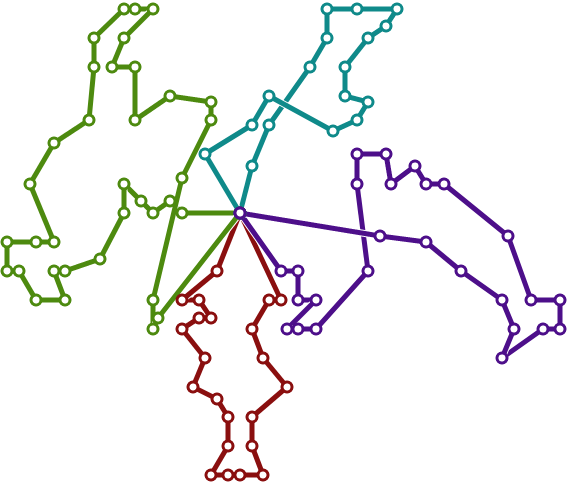
\includegraphics[width=0.7\linewidth]{../article/images/C203-2}
\end{frame}

\begin{frame}
  \frametitle{Décomposition du VRP}

  \begin{itemize}
  \item Séquencement des visites sur un véhicule (Travelling Salesman Problem)
    \begin{itemize}
    \item Vérificateur de contraintes paresseux
    \item Recherche locale (2-opt, \foreign{etc.})
    \end{itemize}
  \item Affectation des visites aux véhicules (Set Packing Problem)
    \begin{itemize}
    \item Mouvement simples (ajout d'une visite, suppression d'une
      visite, déplacement d'une visite)
    \item Choix dans un ensemble d'affectations candidates
    \end{itemize}
  \end{itemize}
\end{frame}

\section{Le voisinage}

\begin{frame}
  \frametitle{Génération des candidats}

  Soit un ensemble de groupes de visites, une tournée candidate est
  une tournée existante à laquelle on peut:

  \begin{itemize}
  \item ne rien changer
  \item enlever un groupe
  \item ajouter un groupe
  \item enlever un groupe et ajouter un groupe
  \end{itemize}

  On obtient un problème de \foreign{set packing} classique, que l'on peut
  facilement résoudre avec un MILP.
\end{frame}

\begin{frame}
  \frametitle{Génération des groupes}

  Classification Ascendante Hiérarchique:
  \begin{itemize}
  \item Distance: intervalle de temps
  \item \foreign{Linkage}: \foreign{single}
  \end{itemize}

  \centering
  \begin{tikzpicture}[scale=0.07]
    \draw<+->[white] (72, 37) -- (98, 48) -- (146, 48) -- (146, 46);
    \draw (35, 0) rectangle (45, 1);
    \draw (62, 0) rectangle (72, 1);
    \draw (78, 0) rectangle (88, 1);
    \draw (98, 0) rectangle (108, 1);
    \draw (136, 0) rectangle (146, 1);
    \draw (172, 0) rectangle (182, 1);

    \draw<+-> (62, 0) -- (62, 26) -- (88, 26) -- (88, 0);
    \draw<+-> (78, 26) -- (78, 30) -- (108, 30) -- (108, 0);
    \draw<+-> (35, 0) -- (35, 37) -- (72, 37) -- (78, 30);
    \draw<+-> (136, 0) -- (136, 46) -- (182, 46) -- (182, 0);
    \draw<+-> (72, 37) -- (98, 48) -- (146, 48) -- (146, 46);
  \end{tikzpicture}
\end{frame}

\begin{frame}
  \frametitle{Quelques mouvements inclus}

  Grâce aux groupes à une visite:

  \begin{itemize}
  \item échange de 2 visites entre 2 tours
  \item rotations de $n$ visites entre $n$ tours
  \item déplacement en chaîne de $n$ visites sur $n+1$ tours
  \end{itemize}

  Grâce aux groupes contenant toutes les visites du tour:

  \begin{itemize}
  \item fusion de 2 tours en un seul
  \end{itemize}

  Grâce à la hiérarchie des groupes:

  \begin{itemize}
  \item répartitions des visites d'un tour sur plusieurs tours
  \item répartitions d'un grand nombre de visites d'un tour sur
    plusieurs tours
  \item des combinaisons de tous ça
  \end{itemize}
\end{frame}

\section{Expérimentations}

\begin{frame}
  \frametitle{VRPTW: instances 100 visites de Solomon}

  Algorithme GRASP: 10 itérations
  \begin{itemize}
  \item Glouton aléatoire tirage sur les 2 meilleurs insertions
  \item Tant qu'il y a amélioration:
    \begin{itemize}
    \item Descente réaffectation d'une visite
    \item Vaste voisinage
    \end{itemize}
  \end{itemize}

  Résultats:
  \begin{itemize}
  \item C20x: Toujours «optimal» sauf 1 (chemin améliorable)
  \item RC20x: «Optimal» vehicule 4/6, durées dans 3-13\%
  \end{itemize}
\end{frame}

\begin{frame}
  \frametitle{Instance industrielles}

  Quelques résultats:
  \begin{itemize}
  \item meilleurs utilisations des véhicules aux caractéristiques
    différentes (diminution de 20 à 9 ressources sur certaines
    instances)
  \item Fonctionne sur une grande variété de problèmes (P\&D, TW,
    flotte hétérogène, \foreign{etc.})
  \item Efficace même sur les très gros problèmes (à 3000 visites) en
    limitant le nombre de groupes
  \end{itemize}
\end{frame}

\begin{frame}
  \frametitle{VRPTW C203: exemple d'exécution}

  \begin{itemize}
  \item Première solution: minimum local (pas d'amélioration en
    déplaçant une visite)
  \item Méthode d'insertion: meilleure insersion successive, suivi
    d'une recherche locale 2-opt
  \item Durée de génération des candidats: 45s environ
  \item Durée de résolution du \foreign{Set Packing Problem}: 15s environ
  \item Durée totale d'exécution: 5 min
  \end{itemize}
\end{frame}

\begin{frame}
  \frametitle{VRPTW C203: minimum local}

  \centering
  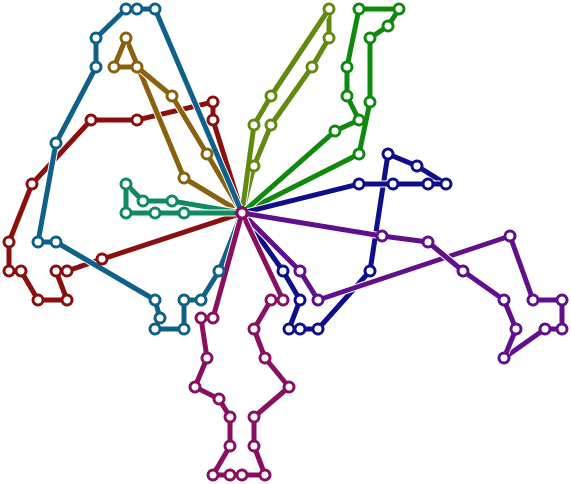
\includegraphics[width=0.7\linewidth]{../article/images/C203-0}
\end{frame}

\begin{frame}
  \frametitle{VRPTW C203: itération 1}

  \centering
  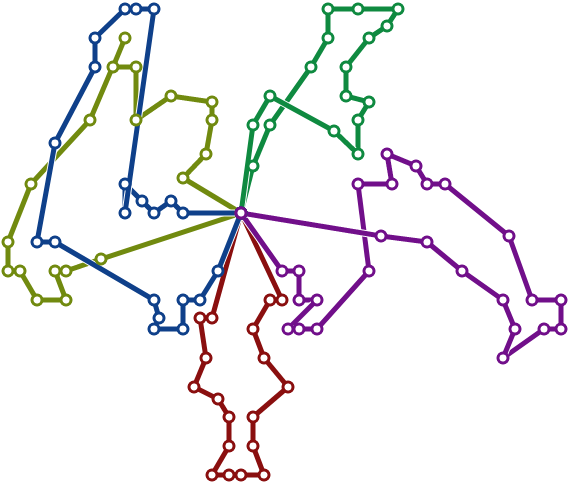
\includegraphics[width=0.7\linewidth]{../article/images/C203-1}
\end{frame}

\begin{frame}
  \frametitle{VRPTW C203: itération 2}

  \centering
  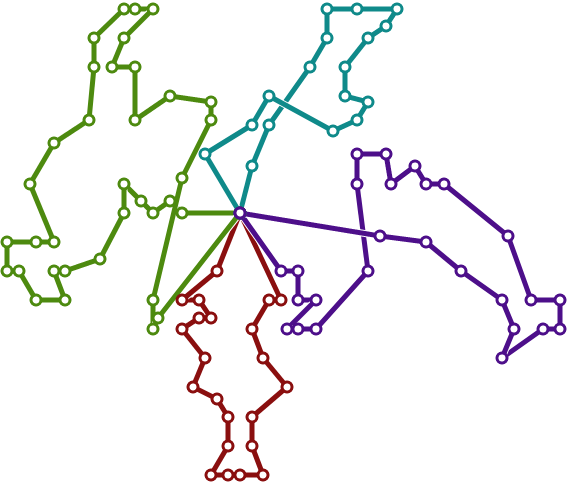
\includegraphics[width=0.7\linewidth]{../article/images/C203-2}
\end{frame}

\begin{frame}
  \frametitle{VRPTW C203: itération 3}

  \centering
  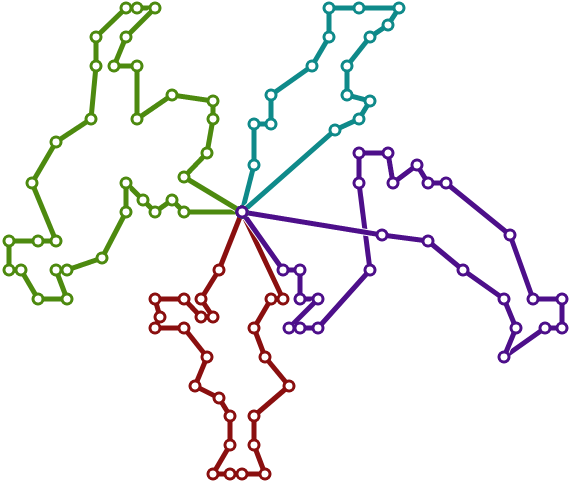
\includegraphics[width=0.7\linewidth]{../article/images/C203-3}
\end{frame}

\begin{frame}
  \frametitle{VRPTW C203: itération 4}

  \centering
  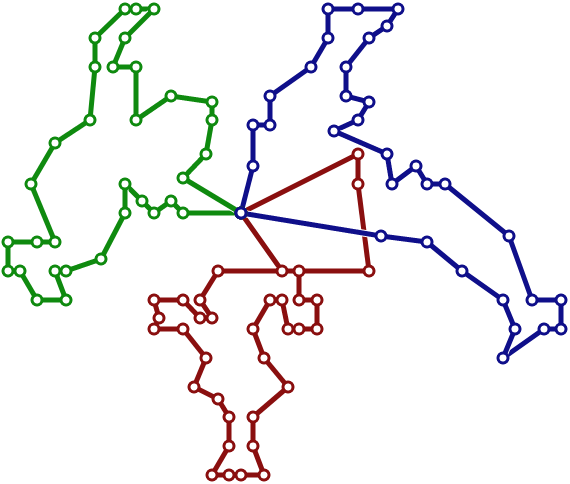
\includegraphics[width=0.7\linewidth]{../article/images/C203-4}
\end{frame}

\begin{frame}
  \frametitle{VRPTW C203: itération 5}

  \centering
  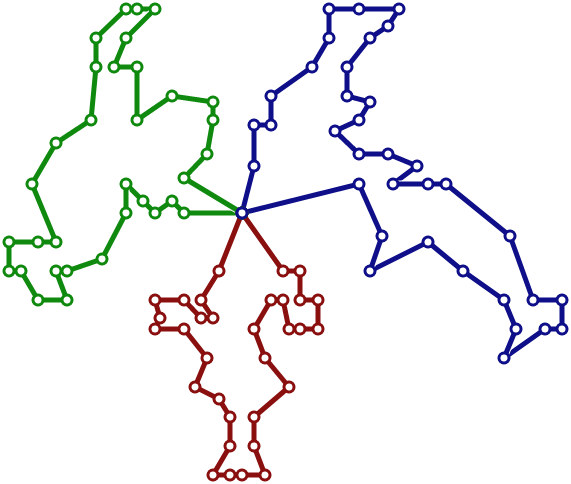
\includegraphics[width=0.7\linewidth]{../article/images/C203-5}
\end{frame}

\section{Conclusion et perspectives}

\begin{frame}
  \frametitle{Conclusions}

  Un nouveau vaste voisinage:
  \begin{itemize}
  \item Flexible et simple
  \item Permet de sortir des minima locaux
  \item Efficace pour minimiser le nombre de véhicules
  \end{itemize}
\end{frame}

\begin{frame}
  \frametitle{Perspectives}

  \begin{itemize}
  \item Explorer différentes méthodes pour générer le regroupement
    hiérarchique:
    \begin{itemize}
    \item métriques
    \item critères de regroupement
    \end{itemize}
  \item Sélectionner un ensemble pertinent de groupes permettant de
    trouver de bonnes solutions
  \end{itemize}
\end{frame}

\begin{frame}
  \titlepage
\end{frame}

\end{document}